\documentclass{article}
\usepackage[UTF8]{ctex} % 用于中文排版
\usepackage{geometry}
\usepackage{indentfirst}
\usepackage{enumitem}

\usepackage{titling}    % 用于自定义标题页
\usepackage{graphicx}
\usepackage{float}

\usepackage{xcolor}
\usepackage{listings}

\usepackage{setspace}

% 页面几何设置
\geometry{a4paper, left=25mm, right=25mm, top=25mm, bottom=25mm}
% 取消首行缩进
\setlength{\parindent}{0pt}
% 行间距设置
\setstretch{1.5}
% 自定义字体大小
\newcommand{\fourhao}{\fontsize{14pt}{\baselineskip}\selectfont} % 四号字体
\newcommand{\xiaosihao}{\fontsize{12pt}{\baselineskip}\selectfont} % 小四号字体
\newcommand{\song}{\CJKfamily{song}}
% 设置代码块格式
\lstset{
    basicstyle = \footnotesize\ttfamily,                 % 设置行距,字体
    numbers = left,                                      % 在左侧显示行号
    numberstyle = \tiny \color{gray},                    % 设定行号格式
    keywordstyle = \bfseries \color[RGB]{40,40,255},     % 设定关键字颜色
    numberstyle = \footnotesize \color{darkgray},           
    commentstyle = \color[RGB]{0,96,96},                 % 设置代码注释的格式
    stringstyle = \color[RGB]{128,0,0},                  % 设置字符串格式
    frame = single,                                      % 不显示背景边框
    backgroundcolor = \color[RGB]{245,245,244},          % 设定背景颜色
    language=Verilog                                     % 设置语言
}
\raggedbottom   % 段落间留白, 避免排版时自动拉伸导致的行间距变化。
\begin{document}

% 封面页面
\begin{titlepage}
    \centering
    \vspace*{2cm}

    \Huge
    \textbf{课程名称:EDA 技术综合设计}

    \vspace{2cm}

    \LARGE
    设计报告名称:设计二\ 数值比较器

    \vspace{4cm}

    \centering
    \Large
    \begin{tabular}{rl}
        班级: & 通信214    \\
        姓名: & \ 王峤宇    \\
        学号: & \ 214022
    \end{tabular}

    \vfill

    \vspace{1cm}
\end{titlepage}

\newpage
% 第一部分
\section*{\fourhao 一、设计内容及原理}
\xiaosihao

% 设计项目内容及设计原理,如真值表、状态表及状态转换图、文字说明等。
\subsection*{基础任务}
\textbf{设计任务}: 首先设计两个一位数值比较器,再设计一个四位数值比较器,输出结果用发光二极管显示即可。\\
一位数值比较器的真值表如表1所示。\\
\begin{table}[H] % 一位数值比较器真值表
    \centering
    \caption{一位比较器真值表}
    \resizebox{6cm}{!}{\begin{tabular}{cc|ccc}
        \hline
        A & B & Above & Equal & Below \\
        \hline \hline
        0&0&0&1&0\\
        0&1&0&0&1\\
        1&0&1&0&0\\
        1&1&0&1&0\\
        \hline
    \end{tabular}}
\end{table}
部分四位数值比较器的真值表如表2所示。\\
\begin{table}[H] % 四位数值比较器真值表
    \centering
    \caption{四位比较器真值表}
    \resizebox{10cm}{!}{\begin{tabular}{cccc|cccc||ccc}
        \hline
        A3 & A2 & A1 & A0 & B3 & B2 & B1 & B0 & Above & Equal & Below \\
        \hline \hline
        1&0&0&0 & 0&x&x&x & 1&0&0\\
        x&1&0&0 & 0&0&x&x & 1&0&0\\
        x&x&1&0 & 0&0&0&x & 1&0&0\\
        x&x&x&1 & 0&0&0&0 & 1&0&0\\
        \hline
        0&x&x&x & 1&0&0&0 & 0&0&1\\
        0&0&x&x & x&1&0&0 & 0&0&1\\
        0&0&0&x & x&x&1&0 & 0&0&1\\
        0&0&0&0 & x&x&x&1 & 0&0&1\\
        \hline
        0&0&0&0 & 0&0&0&0 & 0&1&0\\
        \hline
    \end{tabular}}
\end{table}
针对四位数值比较器, 可以通过观察得知其真值表的规律, 与数值判断同理, 四位数值比较器可以有多个一位数值比较器组成, 
依次从高位开始判断, 最终结果最高位决定, 若前一级的比较器得到了相等的结果则使能下一级比较器进行比较下一位。
\subsection*{提高内容}
\textbf{设计任务}:用一位数值比较器或者四位数值比较器构成一个八位数值比较器,
输出结果用发光二极管显示即可(层次化设计方式)。\\

八位数值比较器构建与四位数值比较器的构建原理相同, 先比较高位, 高位比较器将比较结果传给下一级, 下一级判断输出结果, 
与四位数值比较器用1为数值比较器构成略有不同的地方是, 如果采用四位数值比较器搭建, 该数值比较器需要能够接收来自上一
级的四位数值比较器的输出结果。\\

\begin{figure}[htbp]
    \centering
    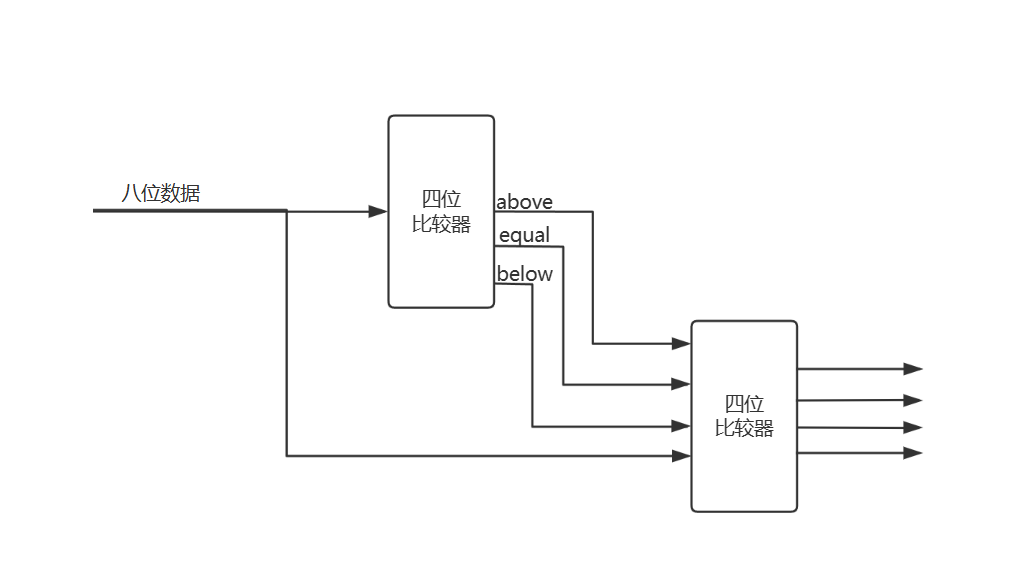
\includegraphics[width=0.7\textwidth]{image/2024-06-28-15-19-27.png}
    \caption{8位数值比较器模块框图}
    \label{image_principle_1}
\end{figure}
八位数值比较器的模块框图如图\ref{image_principle_1}所示。\\
根据此设计的四位数值比较器需要如表3所示的接口。
\begin{table}[htp]
    \centering
    \caption{四位数值比较器接口}
    \resizebox{6cm}{!}{\begin{tabular}{c | c | c}
        \hline
        接口     & 接口类型& 描述\\
        \hline\hline
        A[3:0]   & input  & 数据A\\
        B[3:0]   & input  & 数据B\\ 
        I\_Above & input  & 上级输出\\
        I\_Equal & input  & 上级输出\\
        I\_Below & input  & 上级输出\\
        Y\_Above & output & 输出\\
        Y\_Equal & output & 输出\\
        Y\_Below & output & 输出\\
        \hline
    \end{tabular}}
\end{table}
\subsection*{拓展任务}
\textbf{任务要求}:用一位数值比较器或者四位数值比较器构成一个八位数值比较器,输出结果用发光二极管显示即可
(IP 核设计方式:自己把要用的低位数的数值比较器封装成IP核,然后调用设计八位数值比较器)。\\

该任务任然主要是通过四位数值比较器设计8位数值比较器, 与提高任务在原理上一致。主要是IP核封装的应用。
IP核是指芯片中具有独立功能的电路模块的成熟设计。该电路模块设计可以应用在包含该电路模块的其他芯片设计项目中,
从而减少设计工作量,缩短设计周期,提高芯片设计的成功率, 利用Vivado自带的IP封装工具可以简单的将自己设计并测
试完成的模块进行封装, 供之后调用。
% 第二部分
\setstretch{1.5}
\section*{\fourhao 二、设计过程}
\xiaosihao

% 从工程建立开始,一直到硬件调试。
% 按照基础任务、提高任务和拓展任务分别给出相应的源文件、仿真文件、约束文件
\subsection*{基础任务}
一位数值比较器的源文件如下所示\\
\begin{lstlisting}[language=Verilog, caption={一位数值比较器源文件}]
    module comparator_1bit(
        input a, b,
        output y_above, y_equal, y_below
        );
        assign y_above = a>b ? 1'b1 : 1'b0;      /* 置位a大于b */
        assign y_equal = a==b ? 1'b1 : 1'b0;     /* 置位相等 */
        assign y_below = a<b ? 1'b1 : 1'b0;      /* 置位a小于b */
    endmodule
\end{lstlisting}
一位数值比较器的仿真文件如下所示\\
\begin{lstlisting}[language=Verilog, caption={一位数值比较器测试平台}]
    module comparator_1bit_tb;
    reg   a, b;
    wire  y_above, y_equal, y_below;

    initial begin
        #10;        /* a>b */
        a <= 1'b1;
        b <= 1'b0;
        #10;        /* a=b */
        a <= 1'b1;
        b <= 1'b1;
        #10;        /* a<b */
        a <= 1'b0;
        b <= 1'b1;
        #10;        /* 结束仿真 */
        $finish;
    end
    /* 例化模块 */
    comparator_1bit  comparator_1bit_inst (
        .a(a),
        .b(b),
        .y_above(y_above),
        .y_equal(y_equal),
        .y_below(y_below)
    );
endmodule
\end{lstlisting}
一位数值比较器的用于版上验证的约束文件如下所示, 其中约束文件中, 选择两个拨码开关分别作为输入信号a, b,
选择三个led灯作为输出信号, 查看开发板原理图选择SW7和SW6分别作为a,b, 将LD22~LD20作为三个输出信号, 通过原理图可以得知, LED为高电平点亮, 与逻辑值保持一致。\\
\begin{lstlisting}[language=Verilog, caption={一位数值比较器约束文件}]
set_property PACKAGE_PIN P5 [get_ports a]
set_property IOSTANDARD LVCMOS18 [get_ports a]
set_property PACKAGE_PIN P4 [get_ports b]
set_property IOSTANDARD LVCMOS33 [get_ports b]
set_property PACKAGE_PIN J3 [get_ports y_above]
set_property IOSTANDARD LVCMOS33 [get_ports y_above]
set_property PACKAGE_PIN J2 [get_ports y_equal]
set_property IOSTANDARD LVCMOS33 [get_ports y_equal]
set_property PACKAGE_PIN K2 [get_ports y_below]
set_property IOSTANDARD LVCMOS33 [get_ports y_below]
\end{lstlisting}
四位数值比较器的源文件如下所示\\
\begin{lstlisting}[language=Verilog, caption={四位数值比较器源文件}]
module comparator_4bit(
    input [3:0] a, b,
    input i_above, i_equal, i_below,
    output y_above, y_equal, y_below
    );
    /* 相等时取上一级结果, 不相等则以当前级为输出 */
    assign y_above = a == b ? i_above : (a > b ? 1'b1 : 1'b0);
    /* 相等时, 输出与上级同步 */
    assign y_equal = a == b ? i_equal : 1'b0;
    /* 相等时取上一级结果, 不相等则以当前级为输出 */          
    assign y_below = a == b ? i_below : (a < b ? 1'b1 : 1'b0);
endmodule
\end{lstlisting}
四位数值比较器的仿真文件如下所示\\
\begin{lstlisting}[language=Verilog, caption={四位数值比较器仿真文件}]
module comparator_4bit_tb;
    reg [3:0] a, b;
    reg  i_above, i_equal, i_below;
    wire  y_above, y_equal, y_below;

    initial begin
        {i_above, i_equal, i_below} <= 3'b010;
        #10;        /* a>b */
        a <= 4'd12;
        b <= 4'd11;
        #10;        /* a=b */
        a <= 4'd13;
        b <= 4'd13;
        #10;        /* a<b */
        a <= 4'd8;
        b <= 4'd9;
        #10;        /* 结束仿真 */
        $finish;
    end
    /* 例化四位比较器 */
    comparator_4bit  comparator_4bit_inst (
        .a(a),
        .b(b),
        .i_above(i_above),
        .i_equal(i_equal),
        .i_below(i_below),
        .y_above(y_above),
        .y_equal(y_equal),
        .y_below(y_below)
    );
endmodule
\end{lstlisting}
四位数值比较器的硬件验证约束文件如下所示\\
\begin{lstlisting}[language=Verilog, caption={四位数值比较器的硬件验证约束文件}]
set_property IOSTANDARD LVCMOS33 [get_ports {a[3]}]
set_property IOSTANDARD LVCMOS33 [get_ports {a[2]}]
set_property IOSTANDARD LVCMOS33 [get_ports {a[1]}]
set_property IOSTANDARD LVCMOS33 [get_ports {a[0]}]
set_property IOSTANDARD LVCMOS33 [get_ports {b[3]}]
set_property IOSTANDARD LVCMOS33 [get_ports {b[2]}]
set_property IOSTANDARD LVCMOS33 [get_ports {b[1]}]
set_property IOSTANDARD LVCMOS33 [get_ports {b[0]}]
set_property PACKAGE_PIN J3 [get_ports y_above]
set_property IOSTANDARD LVCMOS33 [get_ports y_above]
set_property PACKAGE_PIN J2 [get_ports y_equal]
set_property IOSTANDARD LVCMOS33 [get_ports y_equal]
set_property PACKAGE_PIN K2 [get_ports y_below]
set_property IOSTANDARD LVCMOS33 [get_ports y_below]

set_property PACKAGE_PIN P5 [get_ports {a[3]}]
set_property PACKAGE_PIN P4 [get_ports {a[2]}]
set_property PACKAGE_PIN P3 [get_ports {a[1]}]
set_property PACKAGE_PIN P2 [get_ports {a[0]}]

set_property PACKAGE_PIN R2 [get_ports {b[3]}]
set_property PACKAGE_PIN M4 [get_ports {b[2]}]
set_property PACKAGE_PIN N4 [get_ports {b[1]}]
set_property PACKAGE_PIN R1 [get_ports {b[0]}]

set_property PACKAGE_PIN U3 [get_ports i_above]
set_property PACKAGE_PIN U2 [get_ports i_equal]
set_property PACKAGE_PIN V2 [get_ports i_below]
set_property IOSTANDARD LVCMOS33 [get_ports i_above]
set_property IOSTANDARD LVCMOS33 [get_ports i_below]
set_property IOSTANDARD LVCMOS33 [get_ports i_equal]
\end{lstlisting}
\subsection*{提高任务}
八位数值比较器采用两个四位数值比较器构成, 其源文件如下所示:
\begin{lstlisting}[language=Verilog, caption={八位数值比较器源文件}]
module comparator_8bit(
    input [7:0] a, b,
    input i_above, i_equal, i_below,
    output y_above, y_equal, y_below
    );

    /* 声明变量, 建立模块间连线 */
    wire above, equal, below;

    /* 例化低位, 第一级比较器 */
    comparator_4bit com0(
        .a(a[3:0]), .b(b[3:0]),
        .i_above(i_above),
        .i_equal(i_equal),
        .i_below(i_below),
        .y_above(above),
        .y_equal(equal),
        .y_below(below)
    );
    /* 例化高位, 第二级比较器 */
    comparator_4bit com1(
        .a(a[7:4]), .b(b[7:4]),
        .i_above(above),
        .i_equal(equal),
        .i_below(below),
        .y_above(y_above),
        .y_equal(y_equal),
        .y_below(y_below)
    );
endmodule
\end{lstlisting}
\begin{lstlisting}[language=Verilog, caption={八位数值比较器Top文件}]
module comparator_8bit_top(
    input [7:0] a, b,
    output y_above, y_equal, y_below
    );
    /* 例化 */
    comparator_8bit  comparator_8bit_inst (
        .a(a), .b(b),
        .i_above(1'b0),
        .i_equal(1'b1),
        .i_below(1'b0),
        .y_above(y_above),
        .y_equal(y_equal),
        .y_below(y_below)
    );
endmodule
\end{lstlisting}    
八位数值比较器的仿真文件如下:
\begin{lstlisting}[language=Verilog, caption={八位数值比较器仿真文件}]
module comparator_8bit_tb;
    reg [7:0] a, b;
    reg  i_above, i_equal, i_below;
    wire  y_above, y_equal, y_below;

    initial begin
        {i_above, i_equal, i_below} <= 3'b010;
        #10;        /* a>b */
        a <= 8'd12;
        b <= 8'd11;
        #10;        /* a<b */
        a <= 8'd8;
        b <= 8'd9;
        #10;        /* a=b */
        a <= 8'd13;
        b <= 8'd13;
        /* 测试级联输入端效果 */
        #10;        /* 上一级(低位)不等, 该级相等 */
        {i_above, i_equal, i_below} <= 3'b100;
        #10;
        $finish;
    end

    comparator_8bit  comp_8bit (
        .a(a),
        .b(b),
        .i_above(i_above),
        .i_equal(i_equal),
        .i_below(i_below),
        .y_above(y_above),
        .y_equal(y_equal),
        .y_below(y_below)
    );
endmodule
\end{lstlisting}

八位数值比较器的硬件验证约束文件如下所示\\
\begin{lstlisting}[language=Verilog, caption={八位数值比较器约束文件}]
set_property IOSTANDARD LVCMOS33 [get_ports {a[3]}]
set_property IOSTANDARD LVCMOS33 [get_ports {a[2]}]
set_property IOSTANDARD LVCMOS33 [get_ports {a[1]}]
set_property IOSTANDARD LVCMOS33 [get_ports {a[0]}]
set_property IOSTANDARD LVCMOS33 [get_ports {b[3]}]
set_property IOSTANDARD LVCMOS33 [get_ports {b[2]}]
set_property IOSTANDARD LVCMOS33 [get_ports {b[1]}]
set_property IOSTANDARD LVCMOS33 [get_ports {b[0]}]
set_property PACKAGE_PIN J3 [get_ports y_above]
set_property IOSTANDARD LVCMOS33 [get_ports y_above]
set_property PACKAGE_PIN J2 [get_ports y_equal]
set_property IOSTANDARD LVCMOS33 [get_ports y_equal]
set_property PACKAGE_PIN K2 [get_ports y_below]
set_property IOSTANDARD LVCMOS33 [get_ports y_below]

set_property PACKAGE_PIN U3 [get_ports i_above]
set_property PACKAGE_PIN U2 [get_ports i_equal]
set_property PACKAGE_PIN V2 [get_ports i_below]
set_property IOSTANDARD LVCMOS33 [get_ports i_above]
set_property IOSTANDARD LVCMOS33 [get_ports i_below]
set_property IOSTANDARD LVCMOS33 [get_ports i_equal]

set_property IOSTANDARD LVCMOS33 [get_ports {a[7]}]
set_property IOSTANDARD LVCMOS33 [get_ports {a[6]}]
set_property IOSTANDARD LVCMOS33 [get_ports {a[5]}]
set_property IOSTANDARD LVCMOS33 [get_ports {a[4]}]
set_property PACKAGE_PIN P5 [get_ports {a[7]}]
set_property PACKAGE_PIN P4 [get_ports {a[6]}]
set_property PACKAGE_PIN P3 [get_ports {a[5]}]
set_property PACKAGE_PIN P2 [get_ports {a[4]}]
set_property PACKAGE_PIN R2 [get_ports {a[3]}]
set_property PACKAGE_PIN M4 [get_ports {a[2]}]
set_property PACKAGE_PIN N4 [get_ports {a[1]}]
set_property PACKAGE_PIN R1 [get_ports {a[0]}]
set_property PACKAGE_PIN U3 [get_ports {b[7]}]
set_property PACKAGE_PIN U2 [get_ports {b[6]}]
set_property PACKAGE_PIN V2 [get_ports {b[5]}]
set_property PACKAGE_PIN V5 [get_ports {b[4]}]
set_property PACKAGE_PIN V4 [get_ports {b[3]}]
set_property PACKAGE_PIN R3 [get_ports {b[2]}]
set_property PACKAGE_PIN T3 [get_ports {b[1]}]
set_property PACKAGE_PIN T5 [get_ports {b[0]}]
set_property IOSTANDARD LVCMOS33 [get_ports {b[7]}]
set_property IOSTANDARD LVCMOS33 [get_ports {b[6]}]
set_property IOSTANDARD LVCMOS33 [get_ports {b[5]}]
set_property IOSTANDARD LVCMOS33 [get_ports {b[4]}]
\end{lstlisting}
\subsection*{拓展任务}
\begin{figure}[H]
    \centering
    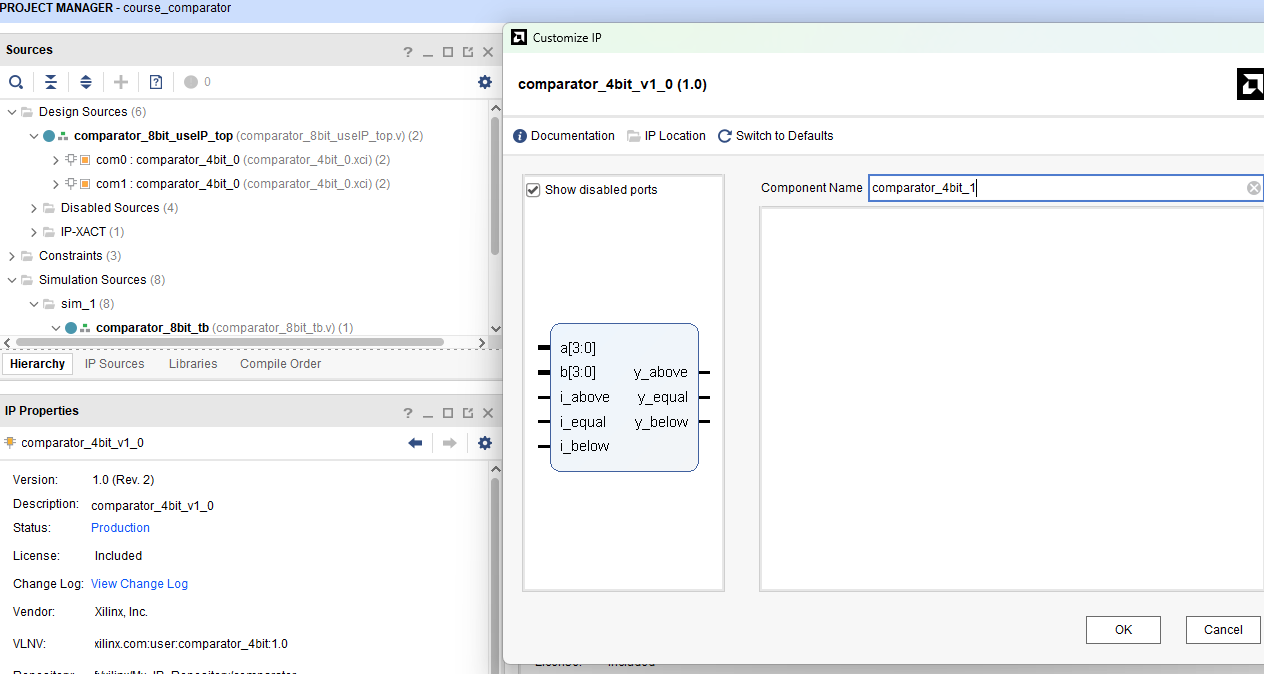
\includegraphics[width=0.7\textwidth]{image/2024-06-15-22-16-36.png}
    \caption{调用四位比较器IP核}
    \label{image_useIP_1}
\end{figure}
通过IP核封装的方式进行8位数值比较器的设计, 调用两个IP核结果如图\ref{image_useIP_1}所示, 使用两个四位比较器。\\
使用IP核的八位数值比较器的源文件Top如下
\begin{lstlisting}[language=Verilog, caption={使用IP核的八位数值比较器的源文件}]
module comparator_8bit_useIP_top(
    input [7:0] a, b,
    output y_above, y_equal, y_below
    );

    wire above, equal, below;
    /* 为IP核配置连接方式, 该四位比较器为第一级 */
    comparator_4bit_0 com0 (
        .a(a[3:0]), .b(b[3:0]),
        .i_above(1'b0),
        .i_equal(1'b1),
        .i_below(1'b0),
        .y_above(above),
        .y_equal(equal),
        .y_below(below)
    );
    /* 为IP核配置连接方式, 该四位比较器为第二级 */
    comparator_4bit_0 com1 (
        .a(a[7:4]), .b(b[7:4]),
        .i_above(above),
        .i_equal(equal),
        .i_below(below),
        .y_above(y_above),
        .y_equal(y_equal),
        .y_below(y_below)
    );
endmodule
\end{lstlisting}
\begin{lstlisting}[language=Verilog, caption={使用IP核的八位数值比较器的仿真文件}]
module comparator_8bit_tb;
    reg [7:0] a, b;
    wire  y_above, y_equal, y_below;

    initial begin
        a <= 8'd44;
        b <= 8'd32;
        #10;        /* a<b */
        a <= 8'd111;
        b <= 8'd192;
        #10;        /* a=b */
        a <= 8'd127;
        b <= 8'd127;
        /* 测试级联输入端效果 */
        #10;        /* 上一级(低位)不等, 该级相等 */
        $finish;
    end

    comparator_8bit_useIP_top  comp_8bit (
        .a(a),
        .b(b),
        .y_above(y_above),
        .y_equal(y_equal),
        .y_below(y_below)
    );
endmodule
\end{lstlisting}
\textbf{约束文件与直接例化使用两个四位数值比较器一致, 不再重复}
% 第三部分
\section*{\fourhao 三、仿真结果}
\xiaosihao
\setstretch{1.5}
% 对仿真图像要有解释,要对所有的可能性进行标注及解释
% 按照基础任务、提高任务和拓展任务分别给出仿真结果
\subsection*{基础任务}
\begin{figure}[H]
    \centering
    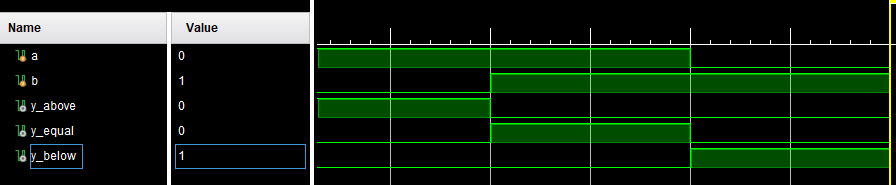
\includegraphics[width=0.7\textwidth]{image/2024-06-14-20-08-22.png}
    \caption{一位数值比较器仿真波形}
    \label{image_1bit_sim}
\end{figure}
一位数值比较器的行为仿真结果如图\ref{image_1bit_sim}所示。根据仿真波形图可以看到比较结果完全正确, 当a=1'b1,b=1'b0时输出位a>b, 
第二状态, 当a=1'b1, b=1'b1时输出为y\_equal, 表示二者相等, 当a = 1'b0, b=1'b1时输出y\_below, 表示a<b。\\
\begin{figure}[H]
    \centering
    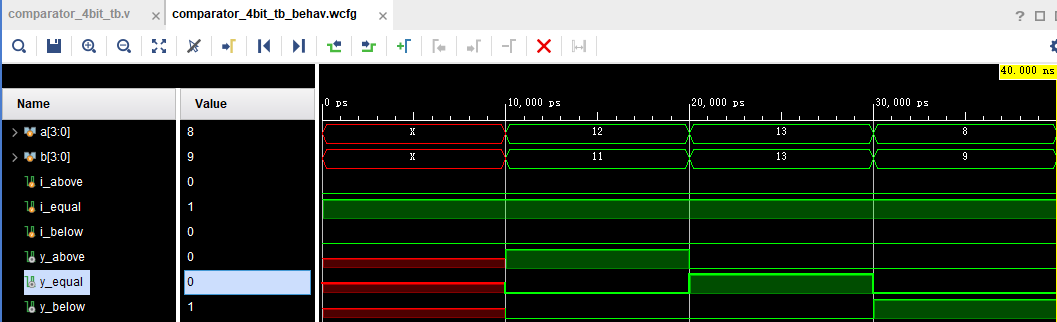
\includegraphics[width=0.7\textwidth]{image/2024-06-15-20-28-49.png}
    \caption{四位数值比较器仿真结果}
    \label{image_4bit_sim}
\end{figure}
四位数值比较器的行为仿真结果如图\ref{image_4bit_sim}所示, 根据仿真波形图可以看到比较结果完全正确, 首先可以看到上一级输入将相等置位1, 其余置位0, 则该模块的输出只受到当前级别的输出, 
测试了三个状态的输入, 当a=12, b=11时,可以正确的检测为a>b, a=13, b=13时,可以正确的检测为a=b, 当a=8, b=9时可以正确的检测到a<b。
\subsection*{提高任务}
\begin{figure}[H]
    \centering
    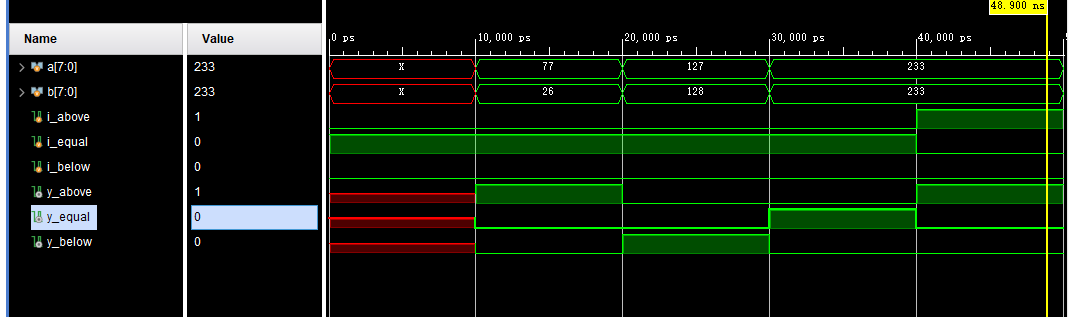
\includegraphics[width=0.7\textwidth]{image/2024-06-15-21-15-24.png}
    \caption{八位数值比较器仿真结果}
    \label{image_8bit_sim}
\end{figure}
八位数值比较器的行为仿真结果如图\ref{image_8bit_sim}所示, 与之前不同的时, 这次对级联输入端进行了测试, 级联输入端能够正常工作, 当本级相等时, 输出结果由更低位决定, 即上一级, 最后一个状态中, 本级比较结果相等, 上一级结果是大于, 所以输出大于, 正确工作。\\
\subsection*{拓展任务}
\begin{figure}[H]
    \centering
    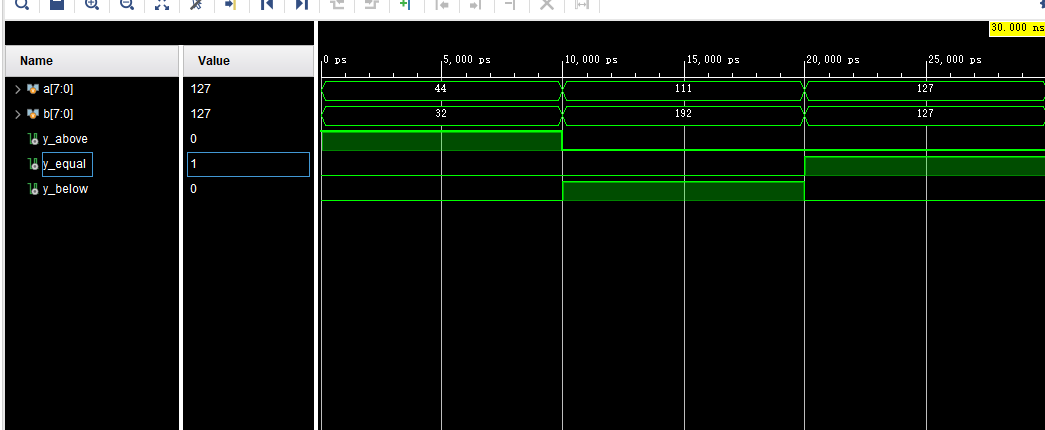
\includegraphics[width=0.7\textwidth]{image/2024-06-15-22-19-35.png}
    \caption{使用四位比较器IP核搭建的八位数值比较器仿真结果}
    \label{image_useIP_2}
\end{figure}
使用IP核搭建的八位数值比较器仿真结果如图\ref{image_useIP_2}所示, 与直接使用两个四位数值比较器例化的形式相同, 可以正确工作。
% 第四部分
\section*{\fourhao 四、硬件验证结果}
\xiaosihao
\setstretch{1.5}
% 记录加编程器与拨码开关和发光二极管、数码管等的连接情况。记录开发板硬件验证结果,并分析其结果的正确性。
% 按照基础任务、提高任务和拓展任务分别分析
\subsection*{基础任务}
一位数值比较器的硬件验证通过两个拨码开关和三个LED完成, 选择SW7和SW6分别作为a,b, 将LD2\_2, LD2\_1, LD2\_0作为三个输出信号, 
具体连接配置可见相应的io约束文件。\\
\begin{figure}[H]
    \centering
    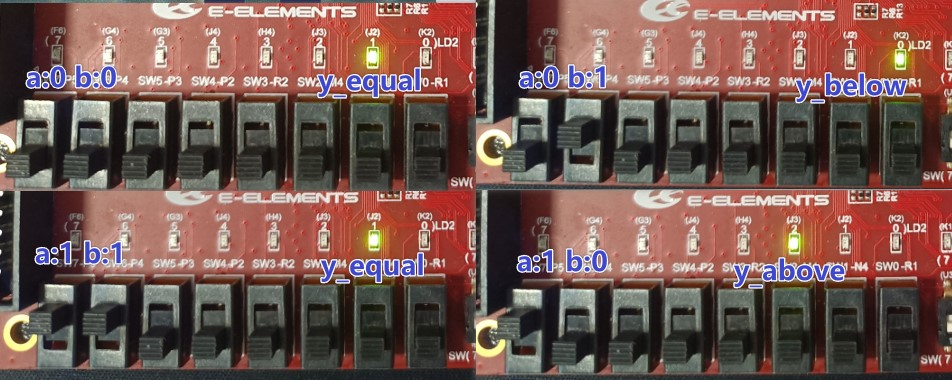
\includegraphics[width=0.7\textwidth]{image/2024-06-14-22-19-02.png}
    \caption{一位数值比较器硬件验证结果}
    \label{image_1bit_verify}
\end{figure}
一位数值比较器硬件验证结果如图\ref{image_1bit_verify}所示, 输出结果对应于输入, 当a=0, b=0或是a=1, b=1时, 模块能够正确识别为相等, 当a=0, b=1时, 可以正确输出a小于b的信号, 相反同理。\\
四位数值比较器的硬件验证与一位数值比较器的输出采用相同的三个LED作为输出信号, 将8个拨码开关作为两个4位二进制输入, SW7-SW4作为a, SW3-SW0作为b。\\
\begin{figure}[H]
    \centering
    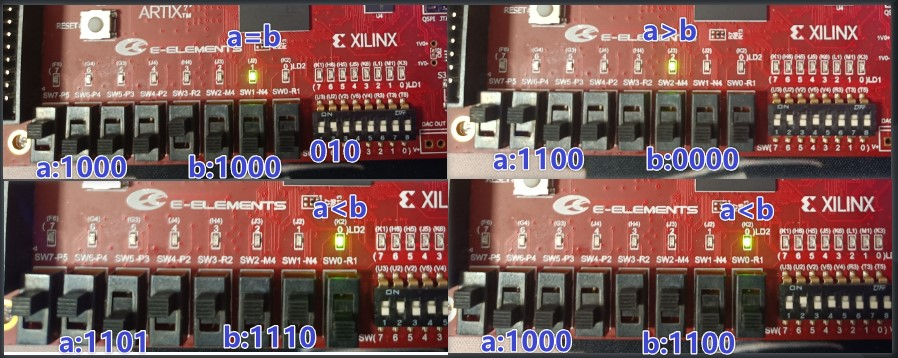
\includegraphics[width=0.7\textwidth]{image/2024-06-15-20-44-19.png}
    \caption{四位数值比较器硬件验证结果}
    \label{image_4bit_verify}
\end{figure}
四位数值比较器硬件验证结果如图\ref{image_4bit_verify}所示, 级联输入端为010, 不使用上一级, 默认将上一级置为相等, 对应于实际比较中低位相等, 高位的比较结果只与高位有关。四次比较结果完全正确。
\subsection*{提高任务}
\begin{figure}[htbp]
    \centering
    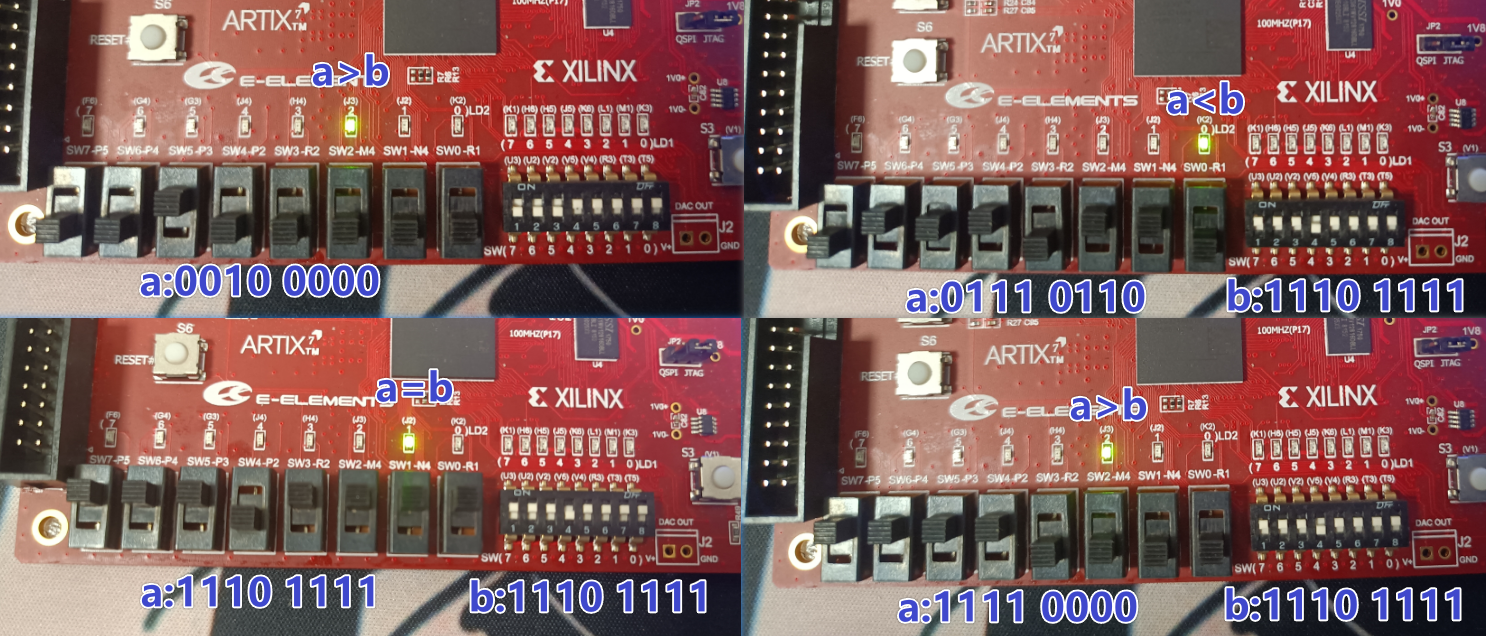
\includegraphics[width=0.7\textwidth]{image/2024-06-15-21-44-16.png}
    \caption{八位数值比较器硬件验证结果}
    \label{image_8bit_verify}
\end{figure}
四位数值比较器硬件验证结果如图\ref{image_8bit_verify}所示, 使用top文件重新例化八位比较器模块, 将级联输入端配置为相等, 实现板上8位数值比较器, 通过拨码开关和八位DIP作为数值输入,
对应于实际比较中低位相等, 高位的比较结果只与高位有关。四次比较结果完全正确, 通过逐位相等判断, 判断IO约束结果无误。
\subsection*{拓展任务}
相比于提高部分的数值比较器, 使用IP核仅仅是改变了模块的构建方式, 对外功能和接口保持一致, 硬件映射相同。同时二者的代码(硬件结构)本质上是一致的, 所以不进行过多测试, 某一次测试结果如图所示。
\begin{figure}[H]
    \centering
    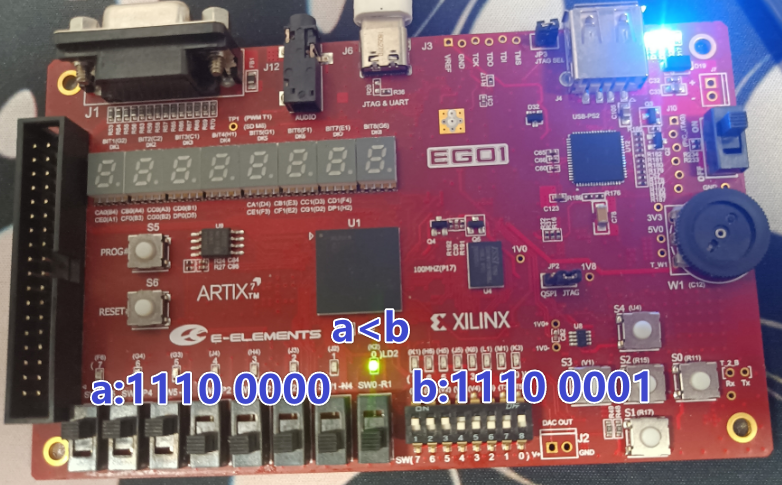
\includegraphics[width=0.7\textwidth]{image/2024-06-15-22-30-05.png}
    \caption{使用IP核构建的八位比较器}
    \label{image_useIP_verify}
\end{figure}
% 第五部分
\section*{\fourhao 五、问题解决}
\xiaosihao
\setstretch{1.5}
% 设计过程中遇到的问题及解决的方法。
\subsection*{调用封装好的IP核后, 综合报错}
解决: 查看报错信息, 报错信息指向了对调用IP核接口配置处, 经过查阅相关资料, 由于自己对IP核调用的错误使用导致。
简单的IP核调用后是直接把对应的源文件导入工程下, 误以为是直接生成对应的模块, 而未进行例化直接使用导致报错。
\subsection*{使用VS Code作为Vivado的编辑器导致Vivado的仿真报错无法进行}
解决: 对现象观察为, 通过Vivado配置编辑器更改后, Vivado默认打开VS Code编写testbench时, 直接在Vivado中进行仿真会无法进行, 会提示文件已被占用, 
针对Vivado的仿真问题有几种方法\\
1. 关闭Vivado自动打开的VS Code界面, 就可以解除占用状态, 进行仿真。\\
2. 手动建立VS Code窗口, 手动配置工作区到Vivado生成的testbench进行编辑, 此时可以在编辑testbench的同时进行Vivado界面的仿真。\\
3. 可以通过VS Code调用第三方仿真工具modelsim完成对Verilog文件的仿真。\\
% 第六部分
\section*{\fourhao 六、心得体会}
\xiaosihao
以较为完整的流程, 包括原理梳理、报告撰写即程序编写和调试完成一次Verilog功能实现, 熟练了对Vivado的使用, 
并通过拓展任务部分的IP核设计任务, 熟悉了Vivado的IP封装工具, 并同时了解了一下Vivado提供的IP核, 如用于
调试的ILA核、常用的时钟核以及FIFO核等。为之后对这些IP核的使用提供了一定的基础。也对EGO1上的外设资源有
了一定的了解, 比如和信号处理相关的DSP模块, 板上FPGA芯片还集成了两个12bit位宽、采样率为1MSPS的XADC, 
可以通过Xilinx提供的IP核直接调用使用。\\

通过完成一个基础组合逻辑电路的实现, 以完全不同的形式实现了在数电课程中, 需要经过真值表、卡诺图化简、
避免竞争和冒险等复杂过程才能设计得到的比较器, 相比之下Verilog实现相同的功能仅需要描述其实现思路, 剩
下的底层门电路的应用全部由计算机计算得到, 也就是综合过程, 感受了EDA设计的强大之处。
\end{document}
